%% Ankur Sinha

%% packages %%
% support for coloured text
\usepackage{xcolor}
% moreland colour palette:
% https://github.com/Gnuplotting/gnuplot-palettes/blob/master/moreland.pal
% create: blue
\definecolor{moreland1}{HTML}{3b4cc0}
%visualise
\definecolor{moreland2}{HTML}{688aef}
%validate
\definecolor{moreland3}{HTML}{99baff}
%simulate
\definecolor{moreland4}{HTML}{c9d8ef}
%fit
\definecolor{moreland5}{HTML}{edd1c2}
%share
\definecolor{moreland6}{HTML}{f7a789}
%reuse
\definecolor{moreland7}{HTML}{e36a53}
% extra: red
\definecolor{moreland8}{HTML}{b40426}

% set 1 colour palette
% https://github.com/Gnuplotting/gnuplot-palettes/blob/master/set1.pal
% red
\definecolor{set11}{HTML}{E41A1C}
% blue
\definecolor{set12}{HTML}{377EB8}
% green
\definecolor{set13}{HTML}{4DAF4A}
% purple
\definecolor{set14}{HTML}{984EA3}
% orange
\definecolor{set15}{HTML}{FF7F00}
% yellow
\definecolor{set16}{HTML}{FFFF33}
% brown
\definecolor{set17}{HTML}{A65628}
% pink
\definecolor{set18}{HTML}{F781BF}

% IPA
\usepackage{tipa}
\usepackage[scale=2]{ccicons}
\usepackage{amssymb}
\usepackage{standalone}
\usepackage{tikz}
\usetikzlibrary{shapes.geometric,arrows,positioning,quotes,graphs,mindmap,decorations.pathmorphing,trees}
\usepackage{jneurosci}
\usepackage{subcaption}
\usepackage[T1]{fontenc}
\usepackage[utf8]{inputenc}
\usepackage[style=nature,backend=biber,autocite=footnote]{biblatex}
\addbibresource{/home/asinha/Documents/01_Readables/00_research_papers/bibliography/masterbib.bib}
\usepackage{roboto}
% for strike through
\usepackage[normalem]{ulem}
% links, urls, refs
\usepackage{hyperref}
\hypersetup{colorlinks,linkcolor=Green,urlcolor=set18}
% graphics
\usepackage{graphicx}
\graphicspath{{99_images/}}
% algorithm
\usepackage{algorithmic}
\usepackage{textcomp}
\usepackage{wrapfig}
\usepackage{textgreek}
\usepackage{euler}
\usepackage{tabularx}
\usepackage{booktabs}
\usepackage{minted}
\usepackage{csquotes}
% beamer theme
% use defaults for theme
\usetheme[progressbar=foot]{moloch}
% for page numbers
\setbeamertemplate{page number in head/foot}[appendixframenumber]
% for footnotes
% https://tex.stackexchange.com/questions/683533/beamer-theme-metropolis-does-not-allow-different-font-size-for-fullcite/683540#683540
\setbeamerfont{bibliography entry title}{size=}
\setbeamerfont{bibliography entry author}{size=}
\setbeamerfont{bibliography entry location}{size=}
\setbeamerfont{bibliography entry note}{size=}
%\usetheme[numbering=fraction,sectionpage=progressbar,subsectionpage=progressbar,progressbar=frametitle]{metropolis}
%\usefonttheme[onlymath]{serif}
\setbeamerfont{footnote}{size=\Tiny}
\setbeamerfont{caption}{size=\tiny}
\setbeamercolor{alerted text}{fg=Green}
\setbeamerfont{note page}{size=\small}
\setbeamercolor{alerted text}{fg=set15}
\setbeamercolor{progress bar}{fg=set18}
\setbeamercolor{title separator}{fg=set18}
\setbeamercolor{frametitle}{bg=moreland1}

\renewcommand{\figurename}{}

% Not needed in metropolis, but in general footnote citation fixes: https://tex.stackexchange.com/questions/44217/how-can-i-stop-footcite-from-hijacking-my-beamer-columns
% how to use multiple references to the same footnote: https://tex.stackexchange.com/questions/27763/beamer-multiple-references-to-the-same-footnote

% Disable footnoterule
\renewcommand{\footnoterule}{}
\renewcommand*{\bibfont}{\tiny}

%% title %%
\title{The NeuroML ecosystem for standardised multi-scale modelling in neuroscience}
\author[Ankur Sinha]{Ankur Sinha\\Silver Lab\\Department of Neuroscience, Physiology, \& Pharmacology\\University College London}
\date{2024-02-26}

%% document begins %%
\begin{document}


% title frame %%
\begin{frame}
  \titlepage{}
\end{frame}
%% Three slides for 5 minutes seems good
%% So, 30 slides at most for 50 minutes

% Why is biophysically detailed modelling important?
% Why are standards necessary?
%\section{Biophysically detailed models and standards}
\begin{frame}[c]
  \frametitle{An understanding of the brain}
  \begin{columns}
    \begin{column}{0.5\textwidth}
      \begin{figure}[h]
        \centering
        \includegraphics[width=\textwidth]{99_images/brain-sizes.jpg}
      \end{figure}
    \end{column}
    \begin{column}{0.5\textwidth}
      \begin{itemize}
        \only<1>{%
          \item<1> \alert{\textasciitilde 86B} neurons
          \item<1> \alert{\textasciitilde 100T} synapses
          \item<1> also \alert{\textasciitilde 85B} glia
        }
        \only<2>{%
          \item<2> specialised \alert{circuits}
          \item<2> different \alert{neuronal} types
          \item<2> \alert{synaptic} connections
          \item<2> complex \alert{sub-cellular} processes
        }
      \end{itemize}
    \end{column}
  \end{columns}
  \vspace{0.2cm}
  \footnotetext[1]{{\tiny{\fullcite{HerculanoHouzel2009}}}}
  \footnotetext[1]{{\tiny{\fullcite{Bartheld2016}}}}
\end{frame}
\note[enumerate]{%
  \item The most recent estimate puts the number of neurons in the human brain at 86B.
  \item Experiments provide us with direct information.
  \item They study the brain at different levels.
  \item There's no right level. It depends on the question being investigated.
}
\begin{frame}[c]
  \frametitle{Experiments provide a window into the brain}
  Multiple scales of experiments/data sources go here
\end{frame}
\note[enumerate]{%
  \item There is so much data out there now, as we embrace Open Science.
}
\begin{frame}[c]
  \frametitle{Models test \& unify experimental results; generate hypotheses}
  \begin{columns}
    \begin{column}{0.5\textwidth}
      \begin{figure}[h]
        \centering
        \includegraphics[width=0.8\textwidth]{99_images/Murray2019-4b}\\\vspace{0.2cm}
        \includegraphics[width=0.9\textwidth]{99_images/TVB}\\
      \end{figure}%
    \end{column}
    \uncover<2>{%
    \begin{column}{0.5\textwidth}
      \begin{figure}[h]
        \centering
        \includegraphics[width=0.65\textwidth]{99_images/20231004-HL23Net}\vspace{0.2cm}
        \includegraphics[width=0.7\textwidth]{99_images/Maeki2020}
      \end{figure}%
    \end{column}}
  \end{columns}
  \footnotetext[1]{\fullcite{Murray2019}}
  \footnotetext[1]{\fullcite{Schirner2023}}
  \footnotetext[1]{\fullcite{Yao2022}}
  \footnotetext[1]{\fullcite{MaekiMarttunen2020}}
\end{frame}
\note[enumerate]{%
\item There is so much data out there now, as we embrace Open Science.
\item Models/theory are necessary for:
\item combining independent experimental results into unified theories
\item exploring these complex systems across wider range of conditions
\item generating new testable hypotheses
\item RNNs are appropriate for lots of projects, for example.
\item So are whole brain neural mass models.
\item But, to really understand the underlying mechanisms that give rise to emergent behaviour, we must model the brain at biophysically detailed levels.
}
\begin{frame}[c]
\frametitle{}
\begin{center}
\Large{A \alert{\emph{mechanistic}} understanding of the brain requires \alert{biophysically detailed} modelling}
\end{center}
\end{frame}
\note[enumerate]{%
\item The figure shows a simplified model life cycle. Can be much more complex in practice.
\item Lots of tools out there for each step.
\item But there's are issues---fragmentation, lack of interoperability, so many APIs.
}
\begin{frame}[c]
  \frametitle{The model life cycle}
      \begin{figure}[h]
        \centering
        \includegraphics[width=\textwidth]{99_images/ecosystem-no-neuroml}
      \end{figure}
\end{frame}
\note[enumerate]{%
\item The figure shows a simplified model life cycle. Can be much more complex in practice.
\item Ideally, what we want is for all the stages to be connected seamlessly, but this is not true in practice.
\item We create our model, ideally re-using already published components.
\item Then before we simulate our model, we want to validate it in some way.
\item We also want to analyse and visualise our model description before.
\item Then we iteratively simulate and fit our model to data, or to produce a certain behaviour.
\item Finally, we want to publish and openly share the model so others can use it in the future.
}
\begin{frame}[c]
  \frametitle{Computational modelling software ecosystem is fragmented}
  \begin{itemize}
    \item many specialist tools:
      \begin{itemize}
        \item NEURON, NEST, Brian, GENESIS, MOOSE, STEPS, ANNarchy, TVB, LFPy, NeuroLib, EDEN, Arbor, NetPyNE\ldots{}
      \end{itemize}
    \item<2-> but:
      \begin{itemize}
        \item<2-> different APIs, syntax:
          \begin{itemize}
            \item<2-> increased difficulty for users
          \end{itemize}
        \item<3-> not well defined model descriptions:
          \begin{itemize}
            \item<3-> models cannot be validated
          \end{itemize}
        \item<4-> custom machine readable internal representations:
          \begin{itemize}
            \item<4-> cannot be easily inspected/analysed
          \end{itemize}
        \item<5-> ad-hoc utilities:
          \begin{itemize}
            \item<5->  cannot be used with all tools
          \end{itemize}
      \end{itemize}
  \end{itemize}
\end{frame}
\note[enumerate]{%
\item There are a lot of software tools out there for users to pick from, for different levels of modelling, optimisation, analysis.
\item For each stage.
\item But, they aren't designed to work together.
\item They have their own designs, their own APIs, syntax, model representation, and usually their own suite of custom utilities to work with their model representation.
}
\begin{frame}[c]
  \frametitle{}
  \begin{center}
  \Large{Makes computational neuroscience models\\\emph{less}\\\alert{FAIR}\\\alert{(Findable, Accessible, Interoperable, Reusable)}}
  \end{center}
\end{frame}
\note[enumerate]{%
\item This means that for example, a model written in simulator A, say NEURON, cannot just be re-used in another simulator.
\item In fact, because a majority of these tools do not have a well defined model description, even re-using models developed in the same simulator can be quite hard.
\item It takes a lot of human resources to translate/convert models to be able to re-use them.
\item It also makes it very hard to study or analyse these models.
}
\begin{frame}[c]
  \frametitle{Standards enable FAIR neuroscience}
  \begin{columns}
    \begin{column}{0.5\textwidth}
      \begin{figure}[h]
        \centering
        \includegraphics[width=0.8\textwidth]{99_images/incf}\\\vspace{0.2cm}
        \includegraphics[width=0.4\textwidth]{99_images/combine}\\
        \scriptsize{COMBINE}
      \end{figure}%
    \end{column}
    \uncover<2>{%
    \begin{column}{0.5\textwidth}
      \begin{figure}[h]
        \centering
        \includegraphics[width=0.35\textwidth]{99_images/neuroml-logo}\\\vspace{0.5cm}
        \includegraphics[width=0.35\textwidth]{99_images/NWB}\\\vspace{0.2cm}
        \includegraphics[width=0.35\textwidth]{99_images/sbml}\\\vspace{0.2cm}
        \includegraphics[width=0.35\textwidth]{99_images/sedml}
      \end{figure}%
    \end{column}}
  \end{columns}
  \footnotetext[1]{\fullcite{Abrams2022}: \url{https://incf.org}}
  \footnotetext[1]{COmputational Modeling in BIology NEtwork (COMBINE): \url{https://co.mbine.org/}}
\end{frame}
\note[enumerate]{%
\item Now, this isn't a problem unique to computational neuroscience, or even neuroscience.
\item Multiple scientific fields have run into this issue, and the answer that they've all come up with is to standardise.
\item Standards allow the representation of data and models in specific, agreed formats.
\item Once a standard is agreed upon, everyone can target it---tools, representations, utilities.
\item If one knows what the data is going to look like, one can then develop tools and APIs around it.
\item And instead of everyone writing a tool for their own standard, every tool anyone writes for the one standard can be used with everyone's data.
}
%\section{NeuroML}
\begin{frame}[c]
  \frametitle{NeuroML ecosystem supports all stages of the model cycle}
  \begin{figure}[h]
    \centering
    \includegraphics[width=\textwidth]{99_images/ecosystem}
  \end{figure}
\end{frame}
\note[enumerate]{%
\item The idea being that by being the standard, various tools that support various stages of the model life cycle can then work together.
}
\begin{frame}[c]
  \frametitle{NeuroML ecosystem}
  \begin{itemize}
    \item standard/specification
    \item software ecosystem
  \end{itemize}
\end{frame}
\note[enumerate]{%
\item It consists of two components. The specification or the standard, and the software that adhere to this specification.
}
\begin{frame}[t]
  \frametitle{NeuroML schema/standard}
    Model specification (XSD)
    \begin{itemize}
      \item elements
      \item attributes
      \item hierarchical relationships
    \end{itemize}
  \uncover<2>{%
    Dynamics (LEMS)
    \begin{itemize}
      \item dynamical behaviour
    \end{itemize}}
\end{frame}
\note[enumerate]{%
\item The standard itself has two different components.
\item There's the schema, which formally specifies the model description---what elements, attributes are valid, and how they related to each other.
\item The next is the LEMS description of the model---the dynamics. We call this the Component type declaration.
}
\begin{frame}[c]
  \frametitle{NeuroML schema/standard: XSD}
    Way of specifying the structure of an XML document.
    \begin{itemize}
      \item allows defining \alert{types} and \alert{extensions/restrictions} on types to create new types.
    \end{itemize}
    \pause{}
    One can validate a model description against the schema \alert{before simulation}
    \footnotetext[1]{\url{https://www.w3.org/TR/xmlschema-1/}}
\end{frame}
\note[enumerate]{%
\item That's it. We'll see an example now.
}
\begin{frame}[fragile,c]
  \frametitle{NeuroML schema/standard: specification: XSD}
  \begin{center}
    \begin{minted}[breaklines=true,autogobble=True,fontsize=\Tiny]{xml}
<xs:simpleType name="Nml2Quantity_voltage"> <!-- For params with dimension voltage -->
  <xs:restriction base="xs:string">
    <xs:pattern value="-?([0-9]*(\.[0-9]+)?)([eE]-?[0-9]+)?[\s]*(V|mV)"/>
  </xs:restriction>
</xs:simpleType>

<xs:complexType name="Izhikevich2007Cell">
  <xs:annotation>
    <xs:documentation>Cell based on ...>
    </xs:documentation>
  </xs:annotation>
  <xs:complexContent>
    <xs:extension base="BaseCellMembPotCap">
      <xs:attribute name="v0" type="Nml2Quantity_voltage" use="required"/>
      <xs:attribute name="k" type="Nml2Quantity_conductancePerVoltage" use="required"/>
      <xs:attribute name="vr" type="Nml2Quantity_voltage" use="required"/>
      <xs:attribute name="vt" type="Nml2Quantity_voltage" use="required"/>
      <xs:attribute name="vpeak" type="Nml2Quantity_voltage" use="required"/>
      <xs:attribute name="a" type="Nml2Quantity_pertime" use="required"/>
      <xs:attribute name="b" type="Nml2Quantity_conductance" use="required"/>
      <xs:attribute name="c" type="Nml2Quantity_voltage" use="required"/>
      <xs:attribute name="d" type="Nml2Quantity_current" use="required"/>
    </xs:extension>
  </xs:complexContent>
</xs:complexType>
    \end{minted}
  \end{center}
\end{frame}
\note[enumerate]{%
\item The schema is defined as an XSD: XML schema document that formally defines what an XML file can look like.
\item In this example, of a simple cell model, the Izhikevich model, this lists what its attributes are.
\item In programming jargon, we're defining the structure of the class---what parameters/attributes can an instance/object of class contain.
}
\begin{frame}[t]
  \frametitle{NeuroML schema/standard: LEMS}
    Low Entropy Model Specification language
    \begin{itemize}
      \item domain independent
      \item machine readable
      \item allows creation of "Component Types" \alert{(classes)} from which "Components" \alert{(objects)} can be instantiated by providing the necessary parameters
      \item provides a reference implementation/simulator
        \pause{}
      \item but is not aware of the cable equation (required for multi-compartmental neuron models)
    \end{itemize}
    \footnotetext[1]{\fullcite{Cannon2014}}
\end{frame}
\note[enumerate]{%
\item The next is the LEMS description of the model---the dynamics. We call this the Component type declaration.
}
\begin{frame}[fragile,c]
  \frametitle{NeuroML schema/standard: dynamics (LEMS)}
  \begin{center}
    \begin{minted}[breaklines=true,autogobble=True,fontsize=\Tiny]{xml}
    <ComponentType name="izhikevich2007Cell" extends="baseCellMembPotCap"
        description="Cell based ...">

        <Parameter name="v0" dimension="voltage" description="Initial membrane potential"/>

        <!--
        Defined in baseCellMembPotCap:
        <Parameter name="C" dimension="capacitance"/>
        -->
        <Parameter name="k" dimension="conductance_per_voltage"/>

        <Parameter name="vr" dimension="voltage" description="Resting membrane potential"/>
        <Parameter name="vt" dimension="voltage" description="Spike threshold"/>
        <Parameter name="vpeak" dimension="voltage" description="Peak action potential value"/>

        <Parameter name="a" dimension="per_time" description="Time scale of recovery variable u"/>
        <Parameter name="b" dimension="conductance" description="Sensitivity of recovery variable u to subthreshold fluctuations of membrane potential v"/>
        <Parameter name="c" dimension="voltage" description="After-spike reset value of v"/>
        <Parameter name="d" dimension="current" description="After-spike increase to u"/>

        <Attachments name="synapses" type="basePointCurrent"/>

        <Exposure name="u" dimension="current" description="Membrane recovery variable"/>

        <Dynamics><!-- snipped --></Dynamics>

    </ComponentType>
    \end{minted}
  \end{center}
\end{frame}
\note[enumerate]{%
\item Here is the LEMS component type definition, without the dynamics for the moment.
\item What you'll notice is that a lot of it is very similar to the XSD definition.
}
\begin{frame}[fragile,c]
  \frametitle{NeuroML schema/standard: XSD and LEMS}
  \begin{center}
    \begin{minted}[breaklines=true,autogobble=True,fontsize=\Tiny]{xml}
      <xs:attribute name="v0" type="Nml2Quantity_voltage" use="required"/>
      <xs:attribute name="k" type="Nml2Quantity_conductancePerVoltage" use="required"/>
      <xs:attribute name="vr" type="Nml2Quantity_voltage" use="required"/>
      <xs:attribute name="vt" type="Nml2Quantity_voltage" use="required"/>
      <xs:attribute name="vpeak" type="Nml2Quantity_voltage" use="required"/>
      <xs:attribute name="a" type="Nml2Quantity_pertime" use="required"/>
      <xs:attribute name="b" type="Nml2Quantity_conductance" use="required"/>
      <xs:attribute name="c" type="Nml2Quantity_voltage" use="required"/>
      <xs:attribute name="d" type="Nml2Quantity_current" use="required"/>
    \end{minted}
    \begin{minted}[breaklines=true,autogobble=True,fontsize=\Tiny]{xml}
        <Parameter name="v0" dimension="voltage" description="Initial membrane potential"/>
        <Parameter name="k" dimension="conductance_per_voltage"/>
        <Parameter name="vr" dimension="voltage" description="Resting membrane potential"/>
        <Parameter name="vt" dimension="voltage" description="Spike threshold"/>
        <Parameter name="vpeak" dimension="voltage" description="Peak action potential value"/>
        <Parameter name="a" dimension="per_time" description="Time scale of recovery variable u"/>
        <Parameter name="b" dimension="conductance" description="Sensitivity of recovery variable u to subthreshold fluctuations of membrane potential v"/>
        <Parameter name="c" dimension="voltage" description="After-spike reset value of v"/>
        <Parameter name="d" dimension="current" description="After-spike increase to u"/>
    \end{minted}
  \end{center}
\end{frame}
\note[enumerate]{%
\item I've written the attributes/parameters together here so you can see that there's a one-to-one correspondence between the two model descriptions.
}
\begin{frame}[fragile,c]
  \frametitle{NeuroML schema/standard: dynamics (LEMS)}
  \begin{center}
    \begin{minted}[breaklines=true,autogobble=True,fontsize=\Tiny]{xml}
    <ComponentType name="izhikevich2007Cell" extends="baseCellMembPotCap"
        description="Cell based ...">
        <!-- snipped -->
        <Dynamics>
            <StateVariable name="v" dimension="voltage" exposure="v"/>
            <StateVariable name="u" dimension="current" exposure="u"/>

            <DerivedVariable name="iSyn"  dimension="current" exposure="iSyn" select="synapses[*]/i" reduce="add" />

            <DerivedVariable name="iMemb" dimension="current" exposure="iMemb" value="k * (v-vr) * (v-vt) + iSyn - u"/>

            <TimeDerivative variable="v" value="iMemb / C"/>
            <TimeDerivative variable="u" value="a * (b * (v-vr) - u)"/>

            <OnStart>
                <StateAssignment variable="v" value="v0"/>
                <StateAssignment variable="u" value="0"/>
            </OnStart>

            <OnCondition test="v .gt. vpeak">
                <StateAssignment variable="v" value="c"/>
                <StateAssignment variable="u" value="u + d"/>
                <EventOut port="spike"/>
            </OnCondition>

        </Dynamics>
    </ComponentType>
    \end{minted}
  \end{center}
\end{frame}
\note[enumerate]{%
\item Now, this isn't a problem unique to computational neuroscience, or even neuroscience.
}
\begin{frame}[c]
  \frametitle{NeuroML provides a set of curated model elements}
    %% https://www.baeldung.com/cs/latex-flowcharts
% using American english
\documentclass{standalone}
\begin{document}

% scale to fit page. using `small mindmap` overrides all the other styles
\tikzset{root concept/.append style={font={\Huge\bfseries}}}
% make all bold
\tikzset{level 1 concept/.append style={font=\bfseries}}
\tikzset{level 2 concept/.append style={font=\bfseries}}
\tikzset{level 3 concept/.append style={font=\bfseries}}
\tikzset{level 4 concept/.append style={font=\bfseries}}

% for level 1 children, start at 15 degrees and proceed. Looks better.
% scale to fit page as necessary

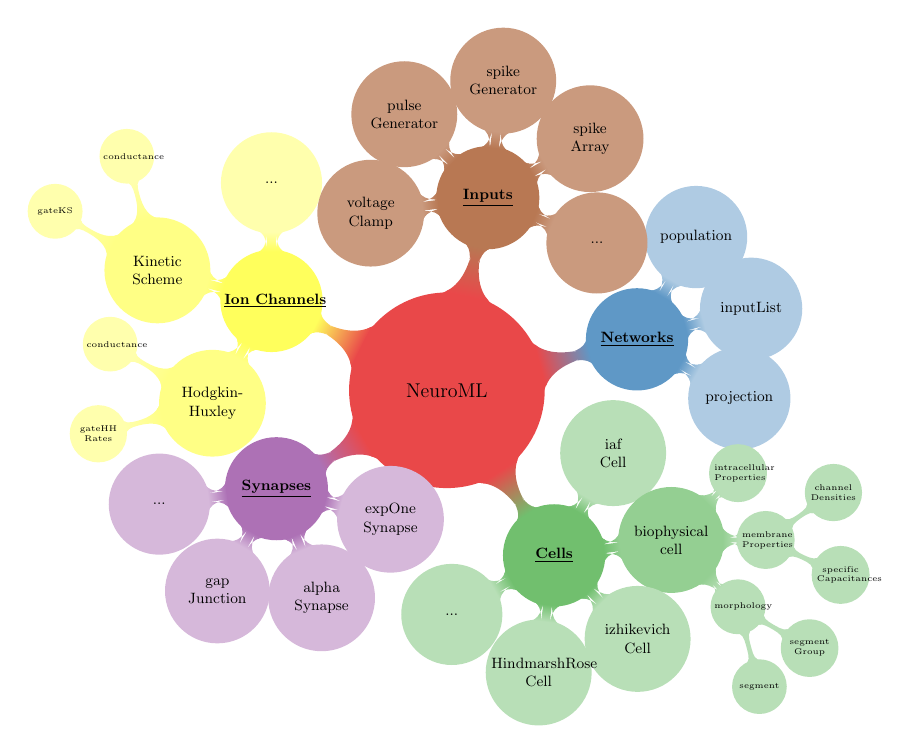
\begin{tikzpicture}[
  mindmap, concept color=set11!80,
  text width=4cm,
  align=flush center,
  scale=0.5, %scale
  every node/.append style={scale=0.6}, %scale
  level 2/.style={level distance=3cm},
  level 4/.style={level distance=2.1cm},
  every concept/.append style={inner sep=1pt, minimum size=0cm},
  decoration={amplitude=0.5cm}
  ]
  \node [concept, circle] {NeuroML}
    child [grow=15, concept color=set12!80] {
      node[concept] {\textbf{\underline{Networks}}}
      [clockwise from=60]
      child [concept color=set12!40, sibling angle=45] {
        node[concept] {population}
      }
      child [concept color=set12!40, sibling angle=45] {
        node[concept] {inputList}
      }
      child [concept color=set12!40, sibling angle=45] {
        node[concept] {projection}
      }
    }
    child [grow=-57, concept color=set13!80] {
      node[concept] {\textbf{\underline{Cells}}}
      [clockwise from=60]
      child [concept color=set13!40, sibling angle=60] {
        node[concept] {iaf\\Cell}
      }
      child [concept color=set13!60, sibling angle=52.5] {
        node[concept] {biophysical\\cell}
        [clockwise from=45]
        child [concept color=set13!40, sibling angle=45] {
          node[concept] {intracellular\\Properties}
        }
        child [concept color=set13!40, sibling angle=45] {
          node[concept] {membrane\\Properties}
          [clockwise from=35]
          child [concept color=set13!40, sibling angle=90] {
            node[concept] {channel\\Densities}
          }
          child [concept color=set13!40, sibling angle=60] {
            node[concept] {specific\\Capacitances}
          }
        }
        child [concept color=set13!40, sibling angle=45] {
          node[concept] {morphology}
          [clockwise from=330]
          child [concept color=set13!40, sibling angle=90] {
            node[concept] {segment\\Group}
          }
          child [concept color=set13!40, sibling angle=45] {
            node[concept] {segment}
          }
        }
      }
      child [concept color=set13!40, sibling angle=52.5] {
        node[concept] {izhikevich\\Cell}
      }
      child [concept color=set13!40, sibling angle=52.5] {
        node[concept] {HindmarshRose\\Cell}
      }
      child [concept color=set13!40, sibling angle=52.5] {
        node[concept] {...}
      }
    }
    child [grow=-150, concept color=set14!80] {
      node[concept] {\textbf{\underline{Synapses}}}
      [clockwise from=-15]
      child [concept color=set14!40, sibling angle=52.5] {
        node[concept] {expOne\\Synapse}
      }
      child [concept color=set14!40, sibling angle=52.5] {
        node[concept] {alpha\\Synapse}
      }
      child [concept color=set14!40, sibling angle=52.5] {
        node[concept] {gap\\Junction}
      }
      child [concept color=set14!40, sibling angle=52.5] {
        node[concept] {...}
      }
    }
    child [grow=-207, concept color=set16!80] {
      node[concept] {\textbf{\underline{Ion Channels}}}
      [clockwise from=240]
      child [concept color=set16!60, sibling angle=60] {
        node[concept] {Hodgkin-Huxley}
        [clockwise from=195]
        child [concept color=set16!40, sibling angle=45, level distance=3cm] {
          node[concept] {gateHH\\Rates}
        }
        child [concept color=set16!40, sibling angle=45, level distance=3cm] {
          node[concept] {conductance}
        }
      }
      child [concept color=set16!60, sibling angle=75] {
        node[concept] {Kinetic Scheme}
        [clockwise from=150]
        child [concept color=set16!40, sibling angle=45, level distance=3cm] {
          node[concept] {gateKS}
        }
        child [concept color=set16!40, sibling angle=45, level distance=3cm] {
          node[concept] {conductance}
        }
      }
      child [concept color=set16!40, sibling angle=75] {
        node[concept] {...}
      }
    }
    child [grow=-282, concept color=set17!80] {
      node[concept] {\textbf{\underline{Inputs}}}
      [clockwise from=187.5]
      child [concept color=set17!60, sibling angle=52.5] {
        node[concept] {voltage\\Clamp}
      }
      child [concept color=set17!60, sibling angle=52.5] {
        node[concept] {pulse\\Generator}
      }
      child [concept color=set17!60, sibling angle=52.5] {
        node[concept] {spike\\Generator}
      }
      child [concept color=set17!60, sibling angle=52.5] {
        node[concept] {spike\\Array}
      }
      child [concept color=set17!60, sibling angle=52.5] {
        node[concept] {...}
      }
    };

\end{tikzpicture}
\end{document}

  \begin{figure}[h]
    \centering
    \includegraphics[width=0.9\textwidth]{99_images/neuroml-mindmap}
  \end{figure}%
\end{frame}
\note[enumerate]{%
\item Now, this isn't a problem unique to computational neuroscience, or even neuroscience.
}
\begin{frame}[c]
  \frametitle{NeuroML is modular, structured and hierarchical}
  \begin{columns}
    \begin{column}{0.3\textwidth}
      \begin{figure}[h]
        \centering
        Conductances\\
        \includegraphics[width=0.7\textwidth]{99_images/membrane2}\\\vspace{0.2cm}
      \end{figure}%
    \end{column}
    \begin{column}{0.3\textwidth}
      \begin{figure}[h]
        \centering
        Cells\\\vspace{-0.5cm}
        \includegraphics[width=0.7\textwidth,angle=-90]{99_images/HL23PYR-red}
        \includegraphics[width=0.7\textwidth,angle=-90]{99_images/HL23PV}
      \end{figure}%
    \end{column}
    \begin{column}{0.3\textwidth}
      \begin{figure}[h]
        \centering
        Networks\\
        \includegraphics[width=0.7\textwidth]{99_images/20231004-HL23Net}\\\vspace{0.2cm}
      \end{figure}%
    \end{column}
  \end{columns}
  \begin{figure}[h]
    \centering
    \includegraphics[width=0.9\textwidth]{99_images/lego}
  \end{figure}%
\end{frame}
\begin{frame}[c]
  \frametitle{NeuroML: software ecosystem}
\begin{figure}[t]
  \begin{figure}[h]
    \centering
    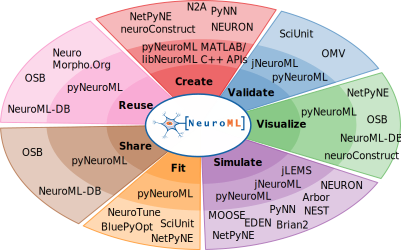
\includegraphics[width=0.9\textwidth]{99_images/ecosystem-onion}
  \end{figure}%
\end{figure}
\end{frame}
\begin{frame}[c]
  \frametitle{NeuroML: software ecosystem: core tools}
  \begin{itemize}
    \item Figure 4
  \end{itemize}
\end{frame}
\begin{frame}[c]
  \frametitle{NeuroML: create models}
  \begin{itemize}
    \item Figure 5
    \item Code example
  \end{itemize}
\end{frame}
\begin{frame}[c]
  \frametitle{NeuroML: validate models}
  \begin{itemize}
    \item Figure 6
  \end{itemize}
\end{frame}
\begin{frame}[c]
  \frametitle{NeuroML: visualise models}
  \begin{itemize}
    \item Figure 7
    \item Figure 8
    \item Figure 9
  \end{itemize}
\end{frame}
\begin{frame}[c]
  \frametitle{NeuroML: simulate models}
  \begin{itemize}
    \item Example simulation: neuron/netpyne
  \end{itemize}
\end{frame}
\begin{frame}[c]
  \frametitle{NeuroML: fit models}
  \begin{itemize}
    \item Figure from docs
    \item Mention inspyred
  \end{itemize}
\end{frame}
\begin{frame}[c]
  \frametitle{NeuroML: share and re-use models}
  \begin{itemize}
    \item GitHub, OSBv1, OSBv2, NeuroML-DB
  \end{itemize}
\end{frame}
%\section{Under the hood}
\begin{frame}[c]
  \frametitle{NeuroML: the APIs}
  \begin{itemize}
    \item Python API
  \end{itemize}
\end{frame}
\begin{frame}[c]
  \frametitle{NeuroML: Documentation}
  \begin{itemize}
    \item Jupyterbook
  \end{itemize}
\end{frame}
\begin{frame}[c]
  \frametitle{NeuroML: projects}
  \begin{itemize}
    \item GSoC, Outreachy, good computer science students
  \end{itemize}
\end{frame}
\begin{frame}[c]
  \frametitle{But, too many standards?}
  \begin{itemize}
    \item XKCD here.
  \end{itemize}
\end{frame}
\note[enumerate]{%
\item In neuroscience, we're fortunate enough to not have the issue of having too many standards.
\item There are only a few standards in biophysically detailed modelling, and as we'll see, we ensure that these few remain interoperable.
}
\end{document}
